% IE 538 Final Presentation - Purdue Black & Old Gold
% Compile with pdflatex
\documentclass[10pt,aspectratio=169]{beamer}

\usepackage{graphicx}
\graphicspath{{figures/}{./}}
\usepackage{booktabs}
\usepackage{amsmath,amssymb}
\usepackage{array}
\usepackage{tikz}
\usetikzlibrary{positioning,shapes,arrows.meta,calc,backgrounds}
\usepackage[T1]{fontenc}
\usepackage{lmodern}

% --- Purdue palette ---
\definecolor{PurdueBlack}{HTML}{000000}
\definecolor{PurdueGold}{HTML}{CEB888}
\definecolor{PurdueDarkGold}{HTML}{8E6F3E}
\definecolor{PurdueGray}{HTML}{555960}
\definecolor{PurdueLightGray}{HTML}{D6D6D6}
\definecolor{AccentRed}{HTML}{B1371B}

% --- Theme setup ---
\usetheme{default}
\usecolortheme{default}
\usefonttheme{professionalfonts}

\setbeamercolor{structure}{fg=PurdueBlack}
\setbeamercolor{title}{fg=PurdueBlack}
\setbeamercolor{frametitle}{fg=PurdueBlack,bg=PurdueGold}
\setbeamercolor{author}{fg=PurdueBlack}
\setbeamercolor{institute}{fg=PurdueGray}
\setbeamercolor{date}{fg=PurdueGray}
\setbeamercolor{block title}{fg=white,bg=PurdueBlack}
\setbeamercolor{block body}{fg=PurdueBlack,bg=PurdueGold!25}
\setbeamercolor{itemize item}{fg=PurdueDarkGold}
\setbeamercolor{itemize subitem}{fg=PurdueGray}
\setbeamercolor{enumerate item}{fg=PurdueDarkGold}
\setbeamercolor{alerted text}{fg=AccentRed}
\setbeamercolor{section in toc}{fg=PurdueBlack}

\setbeamertemplate{itemize item}{\color{PurdueDarkGold}\textbullet}
\setbeamertemplate{itemize subitem}{\color{PurdueGray}\textendash}
\setbeamertemplate{navigation symbols}{}

% Frame title with gold band
\setbeamertemplate{frametitle}{%
  \nointerlineskip%
  \begin{beamercolorbox}[wd=\paperwidth,ht=2.4ex,dp=1ex,leftskip=0.4cm,rightskip=0.4cm]{frametitle}%
    \strut\insertframetitle\strut%
  \end{beamercolorbox}%
}

% Footline: Purdue | short title | page
\setbeamertemplate{footline}{%
  \leavevmode%
  \hbox{%
    \begin{beamercolorbox}[wd=.35\paperwidth,ht=2.4ex,dp=1ex,leftskip=0.4cm]{author in head/foot}%
      \color{PurdueGray}\scriptsize Purdue University $\cdot$ IE 538
    \end{beamercolorbox}%
    \begin{beamercolorbox}[wd=.45\paperwidth,ht=2.4ex,dp=1ex,center]{title in head/foot}%
      \color{PurdueGray}\scriptsize Static Multi-Trip Routing with Nonlinear Inter-Trip Charging
    \end{beamercolorbox}%
    \begin{beamercolorbox}[wd=.2\paperwidth,ht=2.4ex,dp=1ex,center]{date in head/foot}%
      \color{PurdueGray}\scriptsize \insertframenumber\,/\,\inserttotalframenumber
    \end{beamercolorbox}%
  }\vskip2pt%
}

% --- Section divider: full-bleed black page with section title in gold ---
\AtBeginSection[]{%
  {%
  \setbeamercolor{background canvas}{bg=PurdueBlack}%
  \setbeamertemplate{footline}{}%
  \begin{frame}[plain]
    \vfill
    \begin{tikzpicture}[remember picture,overlay]
      \fill[PurdueGold] ([yshift=-3.8cm]current page.west) rectangle ([yshift=-3.4cm]current page.east);
    \end{tikzpicture}
    \begin{center}
      {\scriptsize\color{PurdueGold}\textsc{Section \insertsectionnumber}}\\[6pt]
      {\Huge\bfseries\color{PurdueGold}\insertsection}
    \end{center}
    \vfill
  \end{frame}%
  }%
}

% --- Title info ---
\title{\textbf{Static Multi-Trip Routing \\ and Inter-Trip Charging \\ with Nonlinear Charging Profiles}}
\subtitle{IE 538 Nonlinear Optimization --- Final Project}
\author{Yang Li \and Xiao Li}
\institute{School of Industrial Engineering \\ Purdue University}
\date{April 21, 2026}

\begin{document}

% ================= TITLE =================
{
\setbeamertemplate{footline}{}
\begin{frame}[plain]
\begin{tikzpicture}[remember picture,overlay]
  \fill[PurdueBlack] (current page.north west) rectangle ([yshift=-1.1cm]current page.north east);
  \fill[PurdueGold]  ([yshift=-1.1cm]current page.north west) rectangle ([yshift=-1.3cm]current page.north east);
  \node[anchor=north west,inner sep=0pt,text=PurdueGold]
    at ([xshift=0.6cm,yshift=-0.25cm]current page.north west)
    {\textbf{\large PURDUE}};
  \node[anchor=north east,inner sep=0pt,text=PurdueGold]
    at ([xshift=-0.6cm,yshift=-0.3cm]current page.north west |- current page.north east)
    {\scriptsize IE 538 $\cdot$ Spring 2026};

  \fill[PurdueGold]   (current page.south west) rectangle ([yshift=0.2cm]current page.south east);
  \fill[PurdueBlack]  ([yshift=0.2cm]current page.south west) rectangle ([yshift=0.4cm]current page.south east);
\end{tikzpicture}

\vspace{1.8cm}
\begin{center}
{\huge\bfseries\color{PurdueBlack} Static Multi-Trip Routing \\[2pt]
and Inter-Trip Charging \\[2pt]
with Nonlinear Charging Profiles}\\[12pt]
{\large\color{PurdueGray} IE 538 Nonlinear Optimization --- Final Project}\\[20pt]
{\normalsize\color{PurdueBlack}\textbf{Yang Li} \quad $\cdot$ \quad \textbf{Xiao Li}}\\[6pt]
{\small\color{PurdueGray} School of Industrial Engineering \quad $\cdot$ \quad Purdue University}\\[4pt]
{\small\color{PurdueGray} April 21, 2026}
\end{center}
\end{frame}
}

% ================= AGENDA =================
\begin{frame}{Agenda}
\vspace{6pt}
\begin{columns}[T,onlytextwidth]
\column{0.5\textwidth}
\begin{enumerate}\itemsep5pt
  \item \textbf{Motivation} \\
        {\small\color{PurdueGray} Why charging realism is operationally important.}
  \item \textbf{Problem Setup} \\
        {\small\color{PurdueGray} Static multi-trip E-AFT with inter-trip charging.}
  \item \textbf{Modeling Approach} \\
        {\small\color{PurdueGray} One-stage MIP; PWL charging; indicator coupling.}
\end{enumerate}
\column{0.5\textwidth}
\begin{enumerate}\itemsep5pt
  \setcounter{enumi}{3}
  \item \textbf{Experiments \& Results} \\
        {\small\color{PurdueGray} Direct comparison + symmetric cross-evaluation.}
  \item \textbf{Takeaways} \\
        {\small\color{PurdueGray} When a simplified charging model becomes misleading.}
  \item \textbf{Limitations \& Next Steps}
\end{enumerate}
\end{columns}
\end{frame}

\section{Motivation}

% ================= MOTIVATION =================
\begin{frame}{Why Nonlinear Charging Matters for E-AFT}
\begin{columns}[T,onlytextwidth]
\column{0.58\textwidth}
\textbf{Electrified Autonomous Flexible Transit (E-AFT)}
\begin{itemize}\itemsep3pt
  \item Small batteries $\Rightarrow$ routing is charging-sensitive.
  \item Existing work assumes \alert{constant charging rate} (Jiang et al., 2026).
  \item Real Li-ion batteries \alert{taper}: fast at low SoC, slow at high SoC.
\end{itemize}
\vspace{4pt}
\textbf{Research question}
\begin{block}{}
\emph{Does the charging-rate assumption change \textbf{which passenger requests} an operator chooses to serve --- not just how much charging is performed?}
\end{block}
\column{0.38\textwidth}
\centering
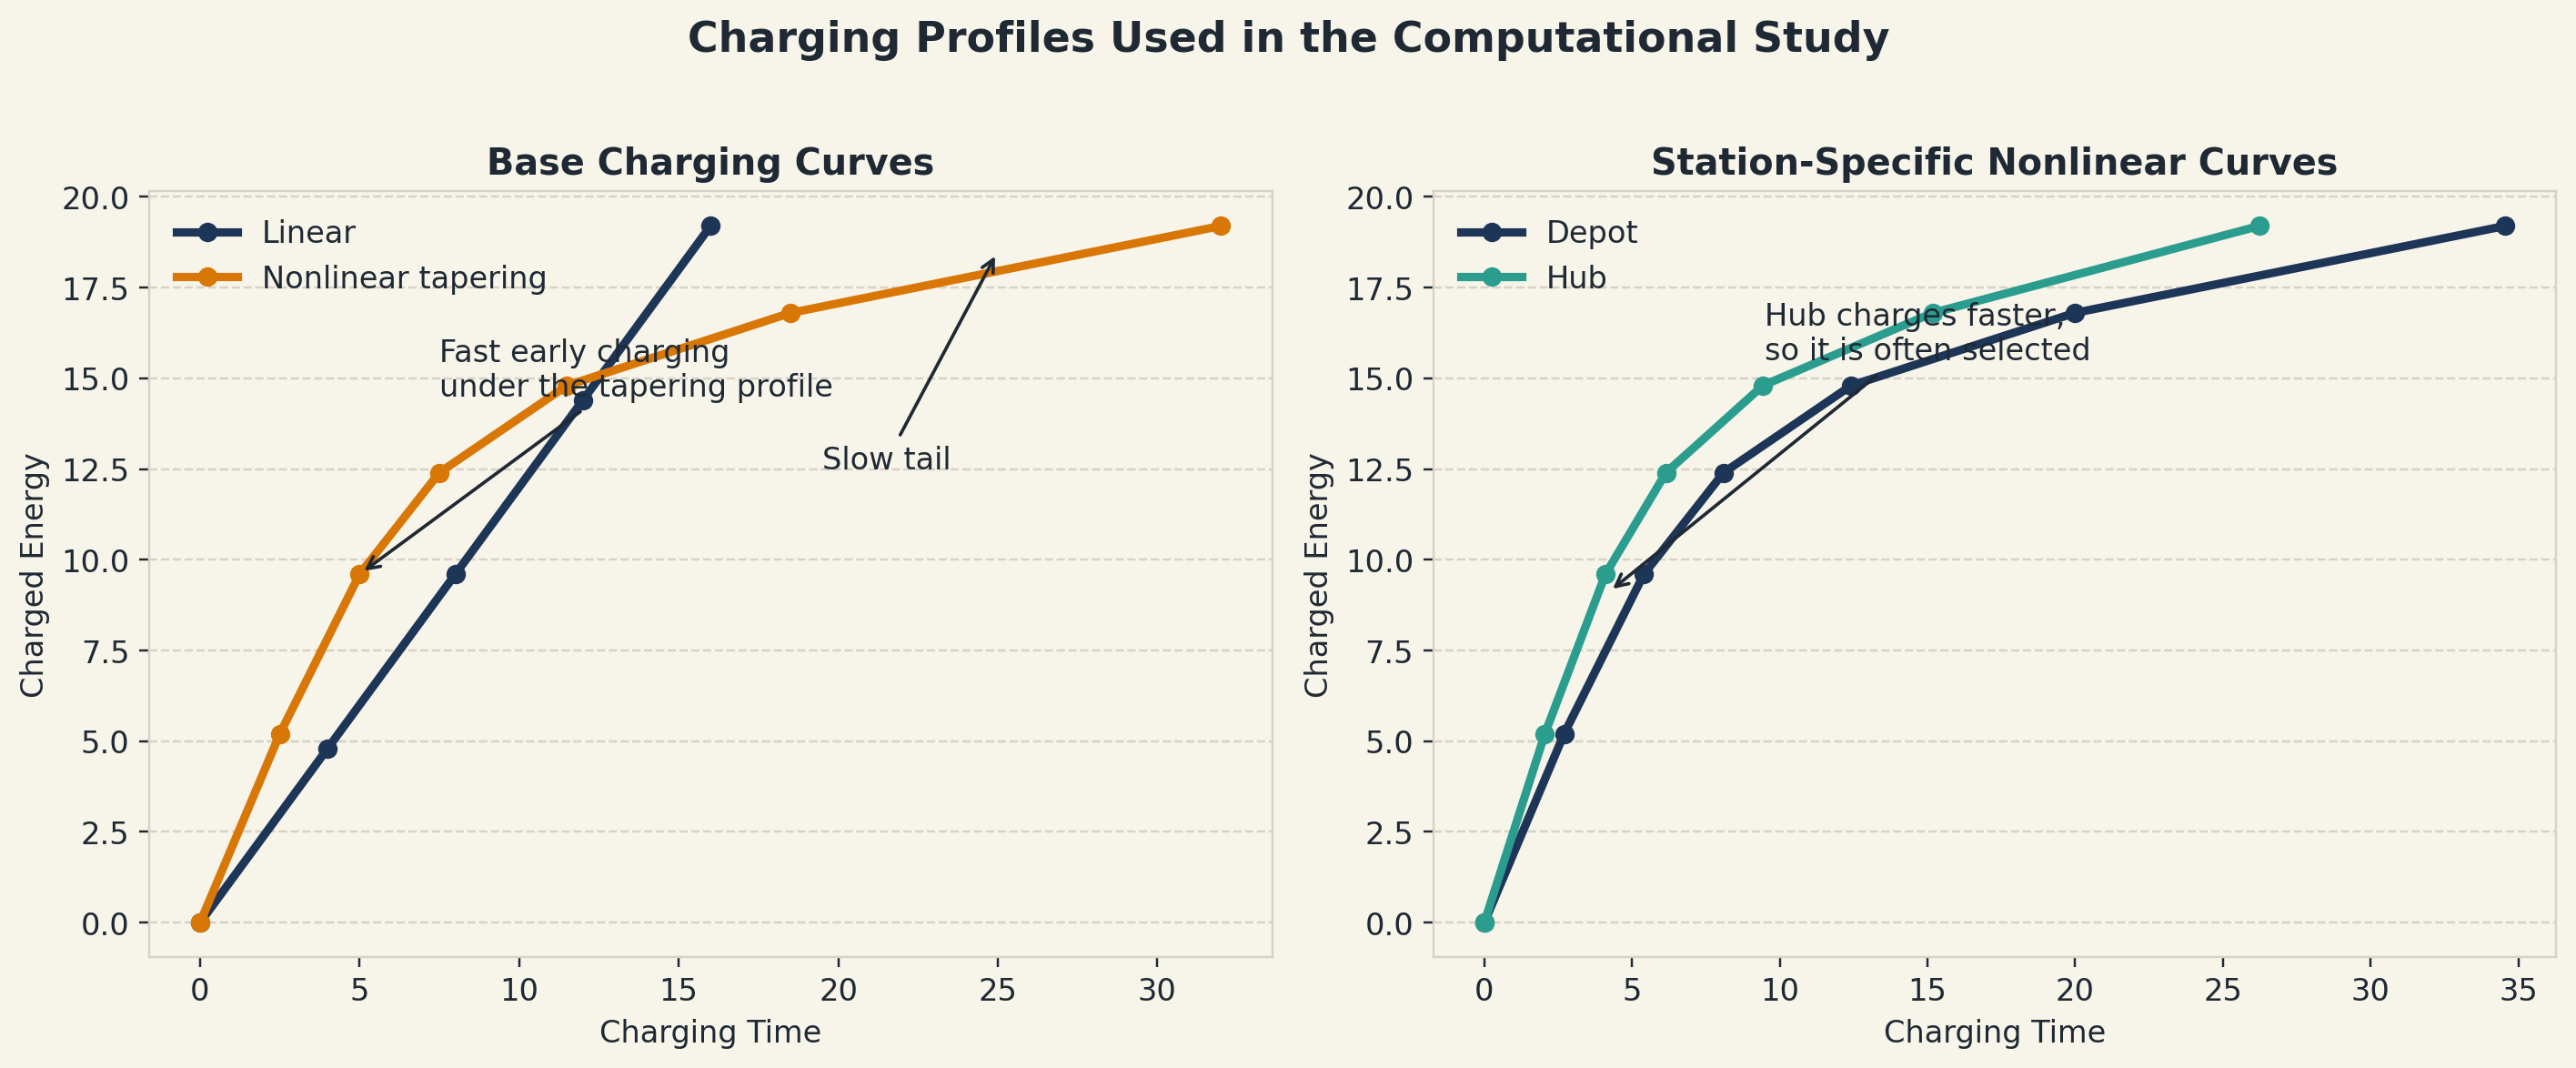
\includegraphics[width=\linewidth]{charging_profiles.png}
\\[2pt]
{\scriptsize Linear vs.\ tapering piecewise-linear charging curves.}
\end{columns}
\end{frame}

\section{Problem Setup}

% ================= PROBLEM SETUP =================
\begin{frame}{E-AFT: The Operating Picture}
\begin{columns}[T,onlytextwidth]
\column{0.55\textwidth}
\textbf{One planning horizon, one bus, multiple trips}
\begin{itemize}\itemsep2pt
  \item Pre-booked passenger requests: origin, destination, pickup time window, \# passengers.
  \item Each trip: a sequence of pickup / drop-off visits, subject to capacity and time windows.
  \item Between consecutive trips: return to a charging station, partial recharge, re-dispatch.
  \item Limited battery $\Rightarrow$ routing, timing, and charging are \emph{tightly coupled}.
\end{itemize}

\vspace{4pt}
\textbf{Decisions (all jointly optimized)}
\begin{itemize}\itemsep1pt
  \item[$\bullet$] Which requests are served, by which trip.
  \item[$\bullet$] Pickup / drop-off order inside each trip.
  \item[$\bullet$] Initial dispatch station; inter-trip station choice.
  \item[$\bullet$] Charging duration \& acquired energy at each station visit.
\end{itemize}

\column{0.43\textwidth}
\centering
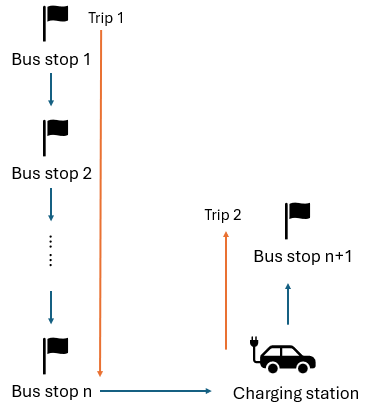
\includegraphics[width=\linewidth]{Figure1.png}\\[4pt]
{\scriptsize A bus cycles through trips of pickups \& drop-offs, returning to a charging station between trips.}
\end{columns}
\end{frame}

% ================= RELATED WORK / POSITIONING =================
\begin{frame}{Where This Project Sits}
\centering\small
\begin{tabular}{@{}p{0.27\textwidth} p{0.33\textwidth} p{0.33\textwidth}@{}}
\toprule
 & \textbf{Jiang et al.\ (2026)} & \textbf{This project} \\
\midrule
Problem scope          & Dynamic routing + charging & \textbf{Static} snapshot of the same problem \\[3pt]
Solution method        & \emph{Two-stage} heuristic decomposition & \textbf{One-stage} integrated MIP \\[3pt]
Charging rate          & \emph{Linear} (constant) & \textbf{Linear vs.\ nonlinear PWL} compared head-to-head \\[3pt]
Station model          & Fixed depot only & Multi-station, per-station speed \emph{and} price \\[3pt]
Dispatch station       & Fixed parameter & \textbf{Decision variable} for the first trip \\[3pt]
Nonlinearity           & Avoided & $E=p\,\theta$ reformulated $\to$ PWL via \texttt{addGenConstrPWL} \\
\bottomrule
\end{tabular}

\vspace{8pt}
\begin{block}{Positioning}
The project's scope is \emph{narrower} than Jiang et al.\ (static, small instances), but it extends their setting in the two directions that matter for a nonlinear-optimization course: \alert{charging-rate nonlinearity} and \alert{joint multi-station charging decisions}.
\end{block}
\end{frame}

\section{Modeling Approach}

% ================= CONTRIBUTIONS =================
\begin{frame}{Contributions}
\begin{enumerate}\itemsep4pt
  \item \textbf{Integrated one-stage MIP}: request selection, trip sequencing, battery propagation, and inter-trip charging solved jointly (vs.\ the two-stage heuristic in Jiang et al., 2026).
  \item \textbf{Multi-station charging} with per-station speed \emph{and} per-station price; and a \textbf{dispatch-station decision variable} for the first trip.
  \item \textbf{Tractable nonlinear charging}: bilinear $E = p\,\theta$ is reformulated as a piecewise-linear map $\theta \mapsto E$ via \texttt{addGenConstrPWL}; station $p$ is absorbed into a time-axis scaling of the PWL breakpoints.
  \item \textbf{Indicator-guarded coupling}: station-off $\Rightarrow$ charge time / energy $=0$ using Gurobi \texttt{addGenConstrIndicator} instead of a loose big-$M$.
  \item \textbf{Symmetric cross-evaluation}: optimize under one charging model, re-evaluate the fixed discrete plan under the other. Both directions tested.
\end{enumerate}
\end{frame}

% ================= MODEL OVERVIEW =================
\begin{frame}{Model --- Objective \& Structure}
\textbf{Objective (primary).} Maximize operating profit:
\vspace{-4pt}
\begin{align*}
Z = \sum_q C_m y_q
  - \sum_q C_z(1\!-\!y_q)
  - \sum_k C_v\,u_k
  - \sum_{k,r} C_t\,u_{kr}
  - C_d \!\!\sum_{k,i,j,r}\!\! \tau_{ij} x_{kijr}
  - \sum_{k,s,r} C_{e,s}\, E_{ksr}.
\end{align*}

\textbf{Hierarchical multi-objective}: profit (priority 2) $>$ total ready/end time (priority 1, tie-breaker).

\vspace{2pt}
\textbf{Constraint families}
\begin{itemize}\itemsep1pt
  \item Request-to-trip assignment, trip activation, subsequent-trip ordering.
  \item Arc-flow routing with in/out degree, first/last node indicators.
  \item Time-window + travel-time propagation on arcs (tightened big-$M$).
  \item Passenger load propagation bounded by $C_b$.
  \item Battery propagation within trips; inter-trip transitions via station.
  \item Charging coupling $E_{ksr} = \mathrm{PWL}_s(\theta_{ksr})$ with station-off indicators.
  \item Symmetry breaking across identical buses.
\end{itemize}
\end{frame}

% ================= CHARGING PWL =================
\begin{frame}{How the Nonlinear Charging Is Modeled}
\begin{columns}[T,onlytextwidth]
\column{0.55\textwidth}
\textbf{From bilinear $E = p\,\theta$ to PWL}
\begin{itemize}\itemsep2pt
  \item Station power $p_s$ is absorbed into a \emph{time-axis} scaling of a shared PWL curve.
  \item Gurobi \texttt{addGenConstrPWL} enforces $E = f_s(\theta)$.
  \item Indicator: $z_{ksr}=0 \Rightarrow \theta_{ksr}=E_{ksr}=0$.
\end{itemize}

\vspace{4pt}
\textbf{Linear curve} (flat 1.2 kWh/min):\\[-8pt]
\[ (0,0),(4,4.8),(8,9.6),(12,14.4),(16,19.2) \]

\textbf{Nonlinear curve} (tapering):\\[-8pt]
\[ \begin{array}{l}
(0,0),(2.5,5.2),(5,9.6),(7.5,12.4),\\
(11.5,14.8),(18.5,16.8),(32,19.2)
\end{array} \]

\scriptsize Segment slopes: $2.08 \to 1.76 \to 1.12 \to 0.60 \to 0.29 \to 0.18$ kWh/min.\\
Station time scale: \texttt{depot} 1.08, \textbf{\texttt{hub} 0.82 (fastest)}, \texttt{edge} 0.93.\\
Station price (\$/kWh): \texttt{depot} 0.48, \texttt{hub} 0.64, \texttt{edge} 0.56.

\column{0.43\textwidth}
\centering
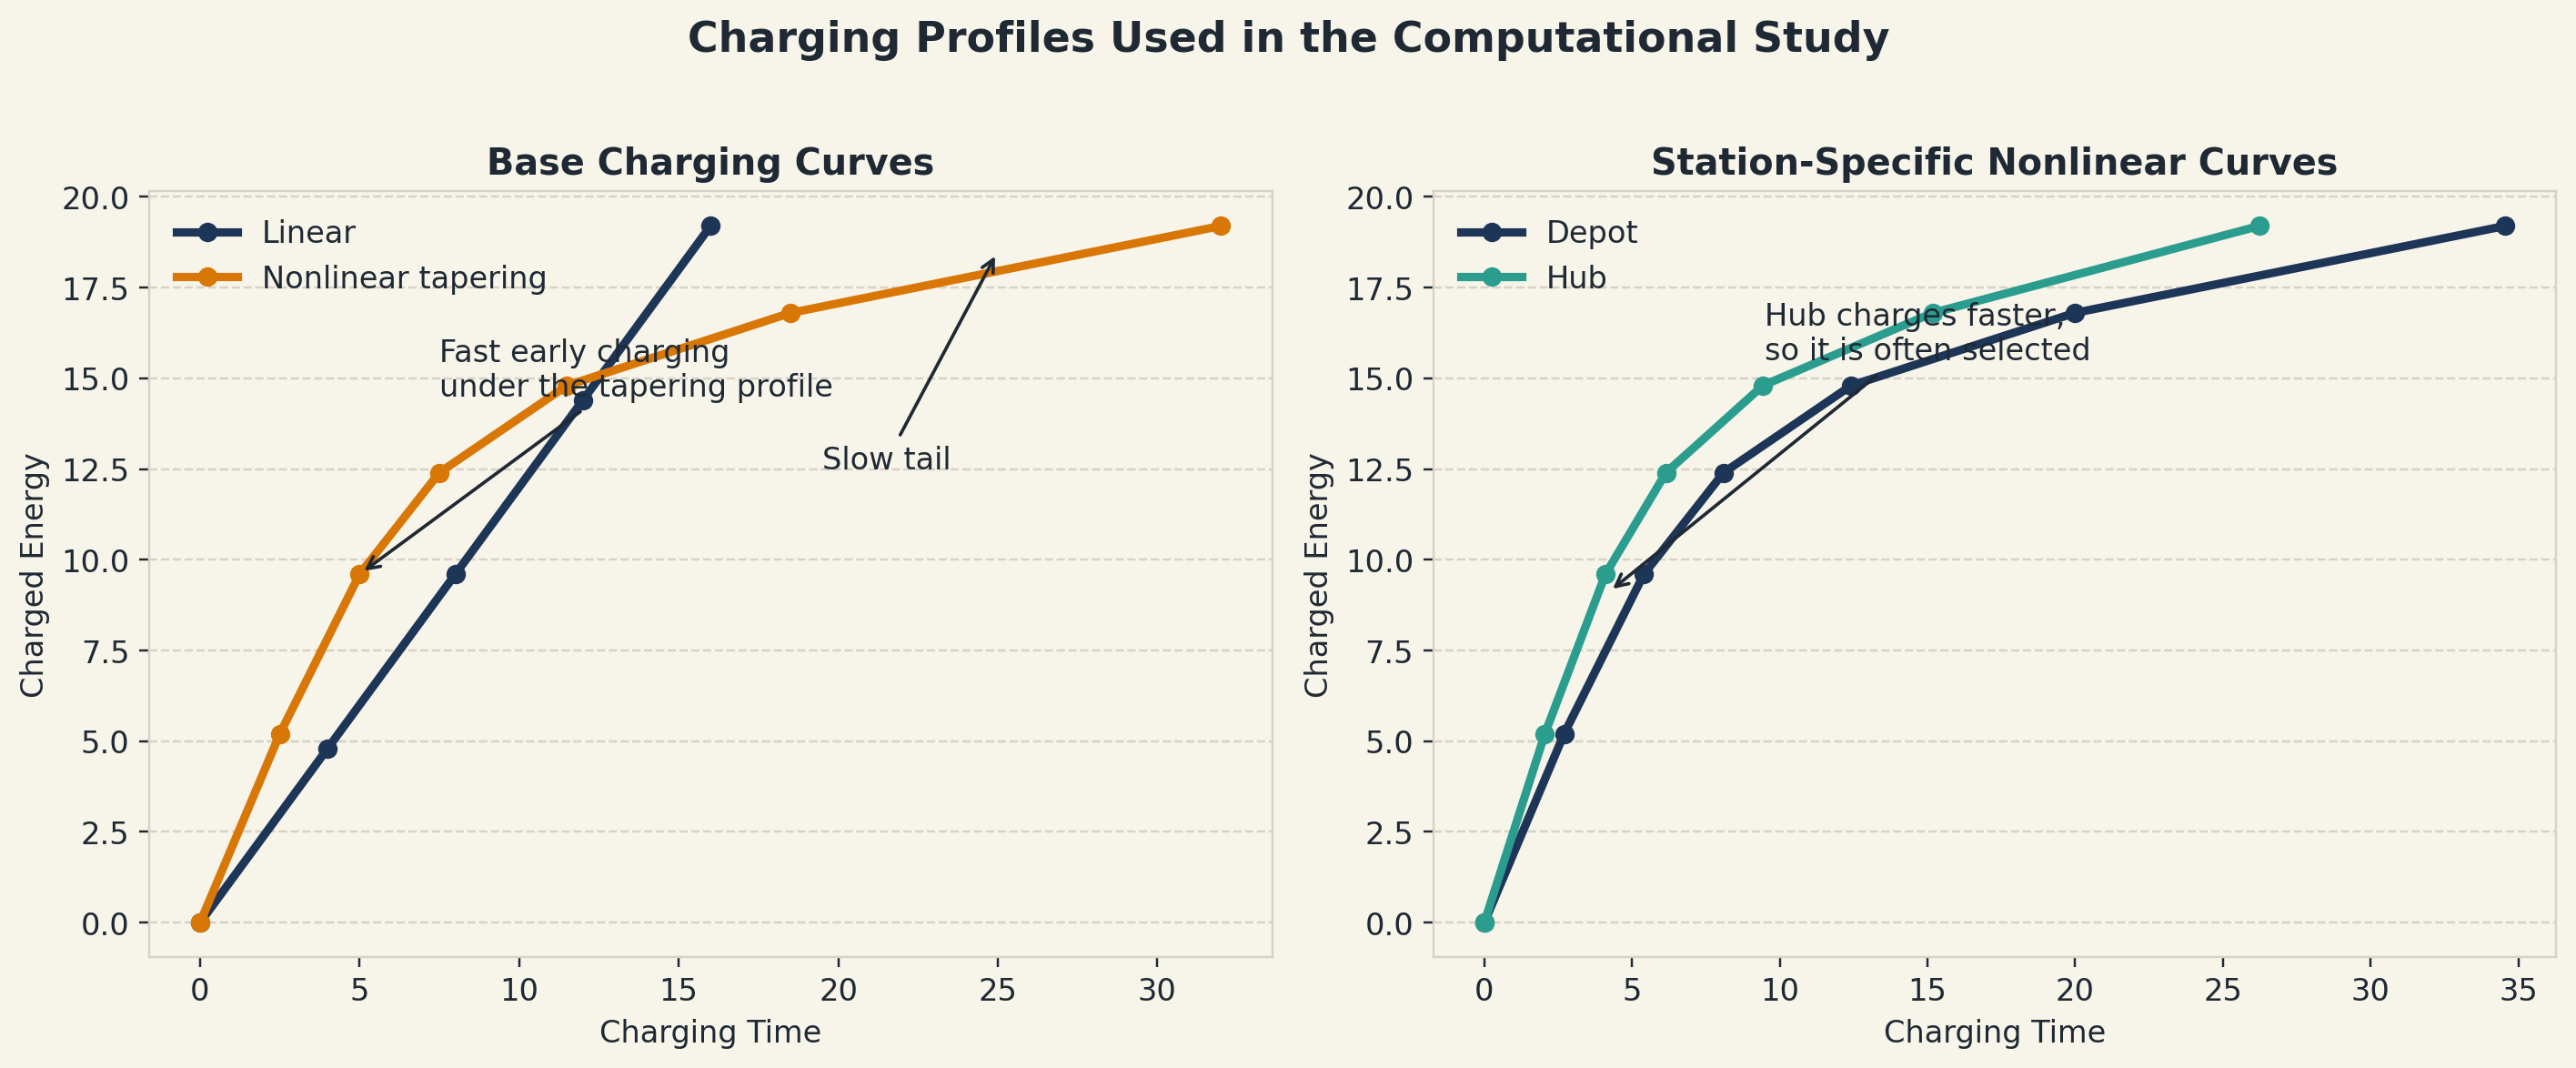
\includegraphics[width=\linewidth]{charging_profiles.png}
\\[2pt]
{\scriptsize Shared-knot PWL; station speed enters via the time-axis scale factor.}
\end{columns}
\end{frame}

\section{Experiments \& Results}

% ================= EXPERIMENTS =================
\begin{frame}{Experimental Design}
\textbf{Setup.} 1 bus, up to 2 trip slots, 2 charging stations, synthetic requests.\\
\textbf{Parameters.} Battery 36 kWh, min 4 kWh, initial 22 kWh, capacity 3 pax. Penalty \$18/unserved.

\vspace{6pt}
\begin{block}{Three diagnostic scenarios}
\begin{tabular}{@{}p{0.19\textwidth}p{0.75\textwidth}@{}}
\textbf{Baseline}       & 4 loose requests; both modes should match (sanity check). \\
\textbf{Partial recharge} & 4 tight requests; a moderate recharge suffices $\Rightarrow$ stresses the fast early portion of the taper. \\
\textbf{Deep recharge}  & 5 requests; the 5th targets a deeper recharge $\Rightarrow$ stresses the flat tail of the taper.
\end{tabular}
\end{block}

\vspace{4pt}
\textbf{Two complementary experiments}
\begin{itemize}\itemsep1pt
  \item \emph{Direct}: solve under each charging model independently.
  \item \emph{Cross-evaluation}: optimize under source mode, fix the discrete plan, re-solve under target mode. Run \emph{both directions} (linear$\to$nonlinear and nonlinear$\to$linear).
\end{itemize}
\end{frame}

% ================= RESULTS TABLE =================
\begin{frame}{Direct Comparison --- Headline Numbers}
\centering
\small
\begin{tabular}{@{}lcccrrc@{}}
\toprule
\textbf{Scenario} & \textbf{R} & \textbf{Mode} & \textbf{Objective} & \textbf{Served} & \textbf{Charge (min / kWh)} \\
\midrule
Baseline          & 4 & Linear     & 202.98 & 4 & 6.95 / 10.17 \\
Baseline          & 4 & Nonlinear  & 202.98 & 4 & 4.52 / 10.17 \\
\rowcolor{PurdueGold!25}
Partial recharge  & 4 & Linear     & 125.99 & 3 & 2.29 / \phantom{0}3.35 \\
\rowcolor{PurdueGold!25}
Partial recharge  & 4 & Nonlinear  & \textbf{202.98} & \textbf{4} & 4.52 / 10.17 \\
Deep recharge     & 5 & Linear     & 184.98 & 4 & 6.95 / 10.17 \\
Deep recharge     & 5 & Nonlinear  & 184.98 & 4 & 4.52 / 10.17 \\
\bottomrule
\end{tabular}

\vspace{10pt}
\begin{columns}[T,onlytextwidth]
\column{0.48\textwidth}
\begin{block}{Baseline}
Both modes serve all 4 requests. Nonlinear still charges faster (4.52 vs 6.95 min) for the \emph{same} 10.17 kWh.
\end{block}
\column{0.48\textwidth}
\begin{block}{Partial recharge --- the headline}
Linear drops \texttt{r4}; nonlinear serves it. \alert{\textbf{+1 request served; +76.99 objective}}.
\end{block}
\end{columns}
\end{frame}

% ================= MECHANISM (the core slide) =================
\begin{frame}{Why Linear Drops \texttt{r4} --- the Arithmetic}
\textbf{Partial-recharge time windows:} \texttt{r3}$\in[43,54]$, \texttt{r4}$\in[55,66]$. Hub time scale 0.82.

\vspace{4pt}
\centering
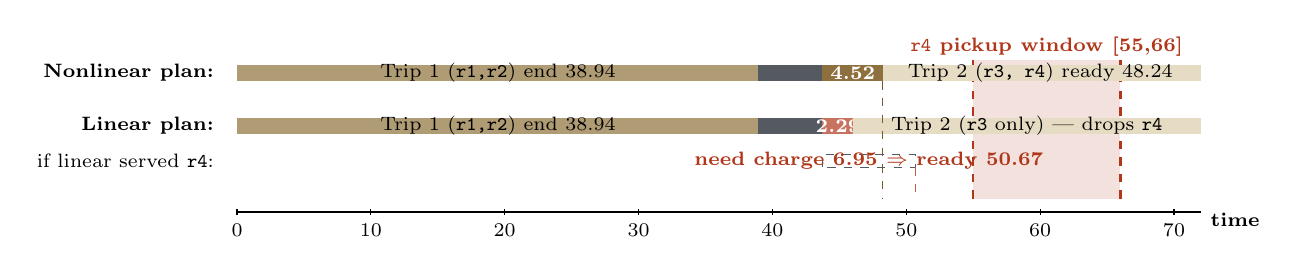
\begin{tikzpicture}[font=\scriptsize,x=0.17cm,y=0.42cm]
% x axis: 1 time unit = 0.2 cm; so 0..72 -> 0..14.4 cm
\draw[thick] (0,0) -- (72,0);
\foreach \t in {0,10,20,30,40,50,60,70}{
  \draw (\t,-0.1) -- (\t,0.1) node[below,yshift=-2pt] {\t};
}
\node[anchor=west,font=\scriptsize\bfseries] at (72,-0.25) {time};

% r4 window [55,66] spanning both rows as a vertical band
\fill[AccentRed!15] (55,0.4) rectangle (66,4.6);
\draw[AccentRed,thick,dashed] (55,0.4) -- (55,4.6);
\draw[AccentRed,thick,dashed] (66,0.4) -- (66,4.6);
\node[text=AccentRed,font=\scriptsize\bfseries] at (60.5,5.0) {\texttt{r4} pickup window [55,66]};

% LINEAR ACTUAL PLAN (y = 2.6): shallow 2.29 charge, trip 2 has r3 only, drops r4
\node[anchor=east,font=\scriptsize\bfseries] at (-1,2.6) {Linear plan:};
\fill[PurdueGold!85!PurdueBlack] (0,2.35) rectangle (38.94,2.85);
\node[font=\scriptsize] at (19.5,2.6) {Trip 1 (\texttt{r1,r2}) end 38.94};
\fill[PurdueGray] (38.94,2.35) rectangle (43.72,2.85);
\fill[AccentRed!70] (43.72,2.35) rectangle (46.01,2.85);
\node[white,font=\scriptsize\bfseries] at (44.9,2.6) {2.29};
\fill[PurdueGold!50] (46.01,2.35) rectangle (72,2.85);
\node[font=\scriptsize] at (59,2.6) {Trip 2 (\texttt{r3} only) --- \alert{drops \texttt{r4}}};

% GHOST BAR: what linear WOULD need to serve r4 (6.95 min charge, trip 2 ready 50.67)
\node[anchor=east,font=\scriptsize] at (-1,1.55) {if linear served \texttt{r4}:};
\draw[PurdueGray,dashed] (43.72,1.35) rectangle (50.67,1.75);
\node[font=\scriptsize\bfseries,text=AccentRed] at (47.2,1.55) {need charge 6.95 $\Rightarrow$ ready 50.67};

% NONLINEAR PLAN (y = 4.2): 4.52 charge, trip 2 serves r3,r4
\node[anchor=east,font=\scriptsize\bfseries] at (-1,4.2) {Nonlinear plan:};
\fill[PurdueGold!85!PurdueBlack] (0,3.95) rectangle (38.94,4.45);
\node[font=\scriptsize] at (19.5,4.2) {Trip 1 (\texttt{r1,r2}) end 38.94};
\fill[PurdueGray] (38.94,3.95) rectangle (43.72,4.45);
\fill[PurdueDarkGold] (43.72,3.95) rectangle (48.24,4.45);
\node[white,font=\scriptsize\bfseries] at (46.0,4.2) {4.52};
\fill[PurdueGold!50] (48.24,3.95) rectangle (72,4.45);
\node[font=\scriptsize] at (60,4.2) {Trip 2 (\texttt{r3, r4}) ready 48.24};

% drop-down guides onto r4 window
\draw[dashed,AccentRed!80]            (50.67,1.35) -- (50.67,0.4);
\draw[dashed,PurdueDarkGold!80!black] (48.24,3.95) -- (48.24,0.4);
\end{tikzpicture}

\vspace{2pt}
\begin{itemize}\itemsep1pt
  \item To serve \{\texttt{r3,r4}\} in Trip 2, Trip 2 needs 10.17 kWh at start.
  \item At the \textbf{constant} hub rate, 10.17 kWh $=$ \alert{6.95 min} $\Rightarrow$ Trip 2 ready $\approx 50.67$ \alert{collides with \texttt{r4}'s [55,66] window after travel}.
  \item Linear therefore \emph{retreats} to a 2.29 min / 3.35 kWh shallow recharge and \emph{drops} \texttt{r4}.
  \item At the \textbf{tapering} rate, same 10.17 kWh $=$ \textbf{4.52 min} $\Rightarrow$ Trip 2 ready 48.24, \textbf{fits}.
\end{itemize}
\end{frame}

% ================= CROSS EVAL =================
\begin{frame}{Cross-Evaluation --- Symmetric Test}
\begin{columns}[T,onlytextwidth]
\column{0.5\textwidth}
\textbf{linear $\to$ nonlinear} (partial recharge)\\
\scriptsize Optimize under linear, fix plan, re-evaluate under nonlinear.
\begin{itemize}\itemsep1pt
  \item[\color{PurdueDarkGold}\textbullet] Fixed plan \textbf{remains feasible}: 125.99.
  \item[\color{PurdueDarkGold}\textbullet] Charging finishes \emph{faster} (1.32 vs 2.29 min).
  \item[\color{AccentRed}\textbullet] \textbf{Free re-optimization} under nonlinear $\Rightarrow$ 202.98 \alert{(+76.99, +1 served request)}.
\end{itemize}

\column{0.5\textwidth}
\textbf{nonlinear $\to$ linear} (partial recharge)\\
\scriptsize Optimize under nonlinear, fix plan, re-evaluate under linear.
\begin{itemize}\itemsep1pt
  \item[\color{AccentRed}\textbf{!}] Fixed plan is \alert{\textbf{INFEASIBLE}}.
  \item[\color{PurdueDarkGold}\textbullet] Why: 10.17 kWh takes 6.95 min under linear, Trip 2 ready slips to 50.67, which (with the return+start legs) blows the \texttt{r4} pickup window.
  \item[\color{PurdueDarkGold}\textbullet] Re-optimization must retreat to the 3-request plan (125.99).
\end{itemize}
\end{columns}

\vspace{6pt}
\begin{block}{The symmetric headline}
A nonlinear-optimal plan \textbf{cannot be executed} under a linear charging assumption --- it is not merely suboptimal, it violates the service time windows. Using a simplified linear model for planning therefore risks promising a plan the physical battery cannot deliver.
\end{block}

\scriptsize Deep recharge ($R=5$): both modes converge on the same 2-trip / 4-served plan; asymmetry only appears once the taper actually binds (partial recharge regime).
\end{frame}

% ================= FIGURES =================
\begin{frame}{Visual Summary of the Results}
\begin{columns}[T,onlytextwidth]
\column{0.5\textwidth}
\centering
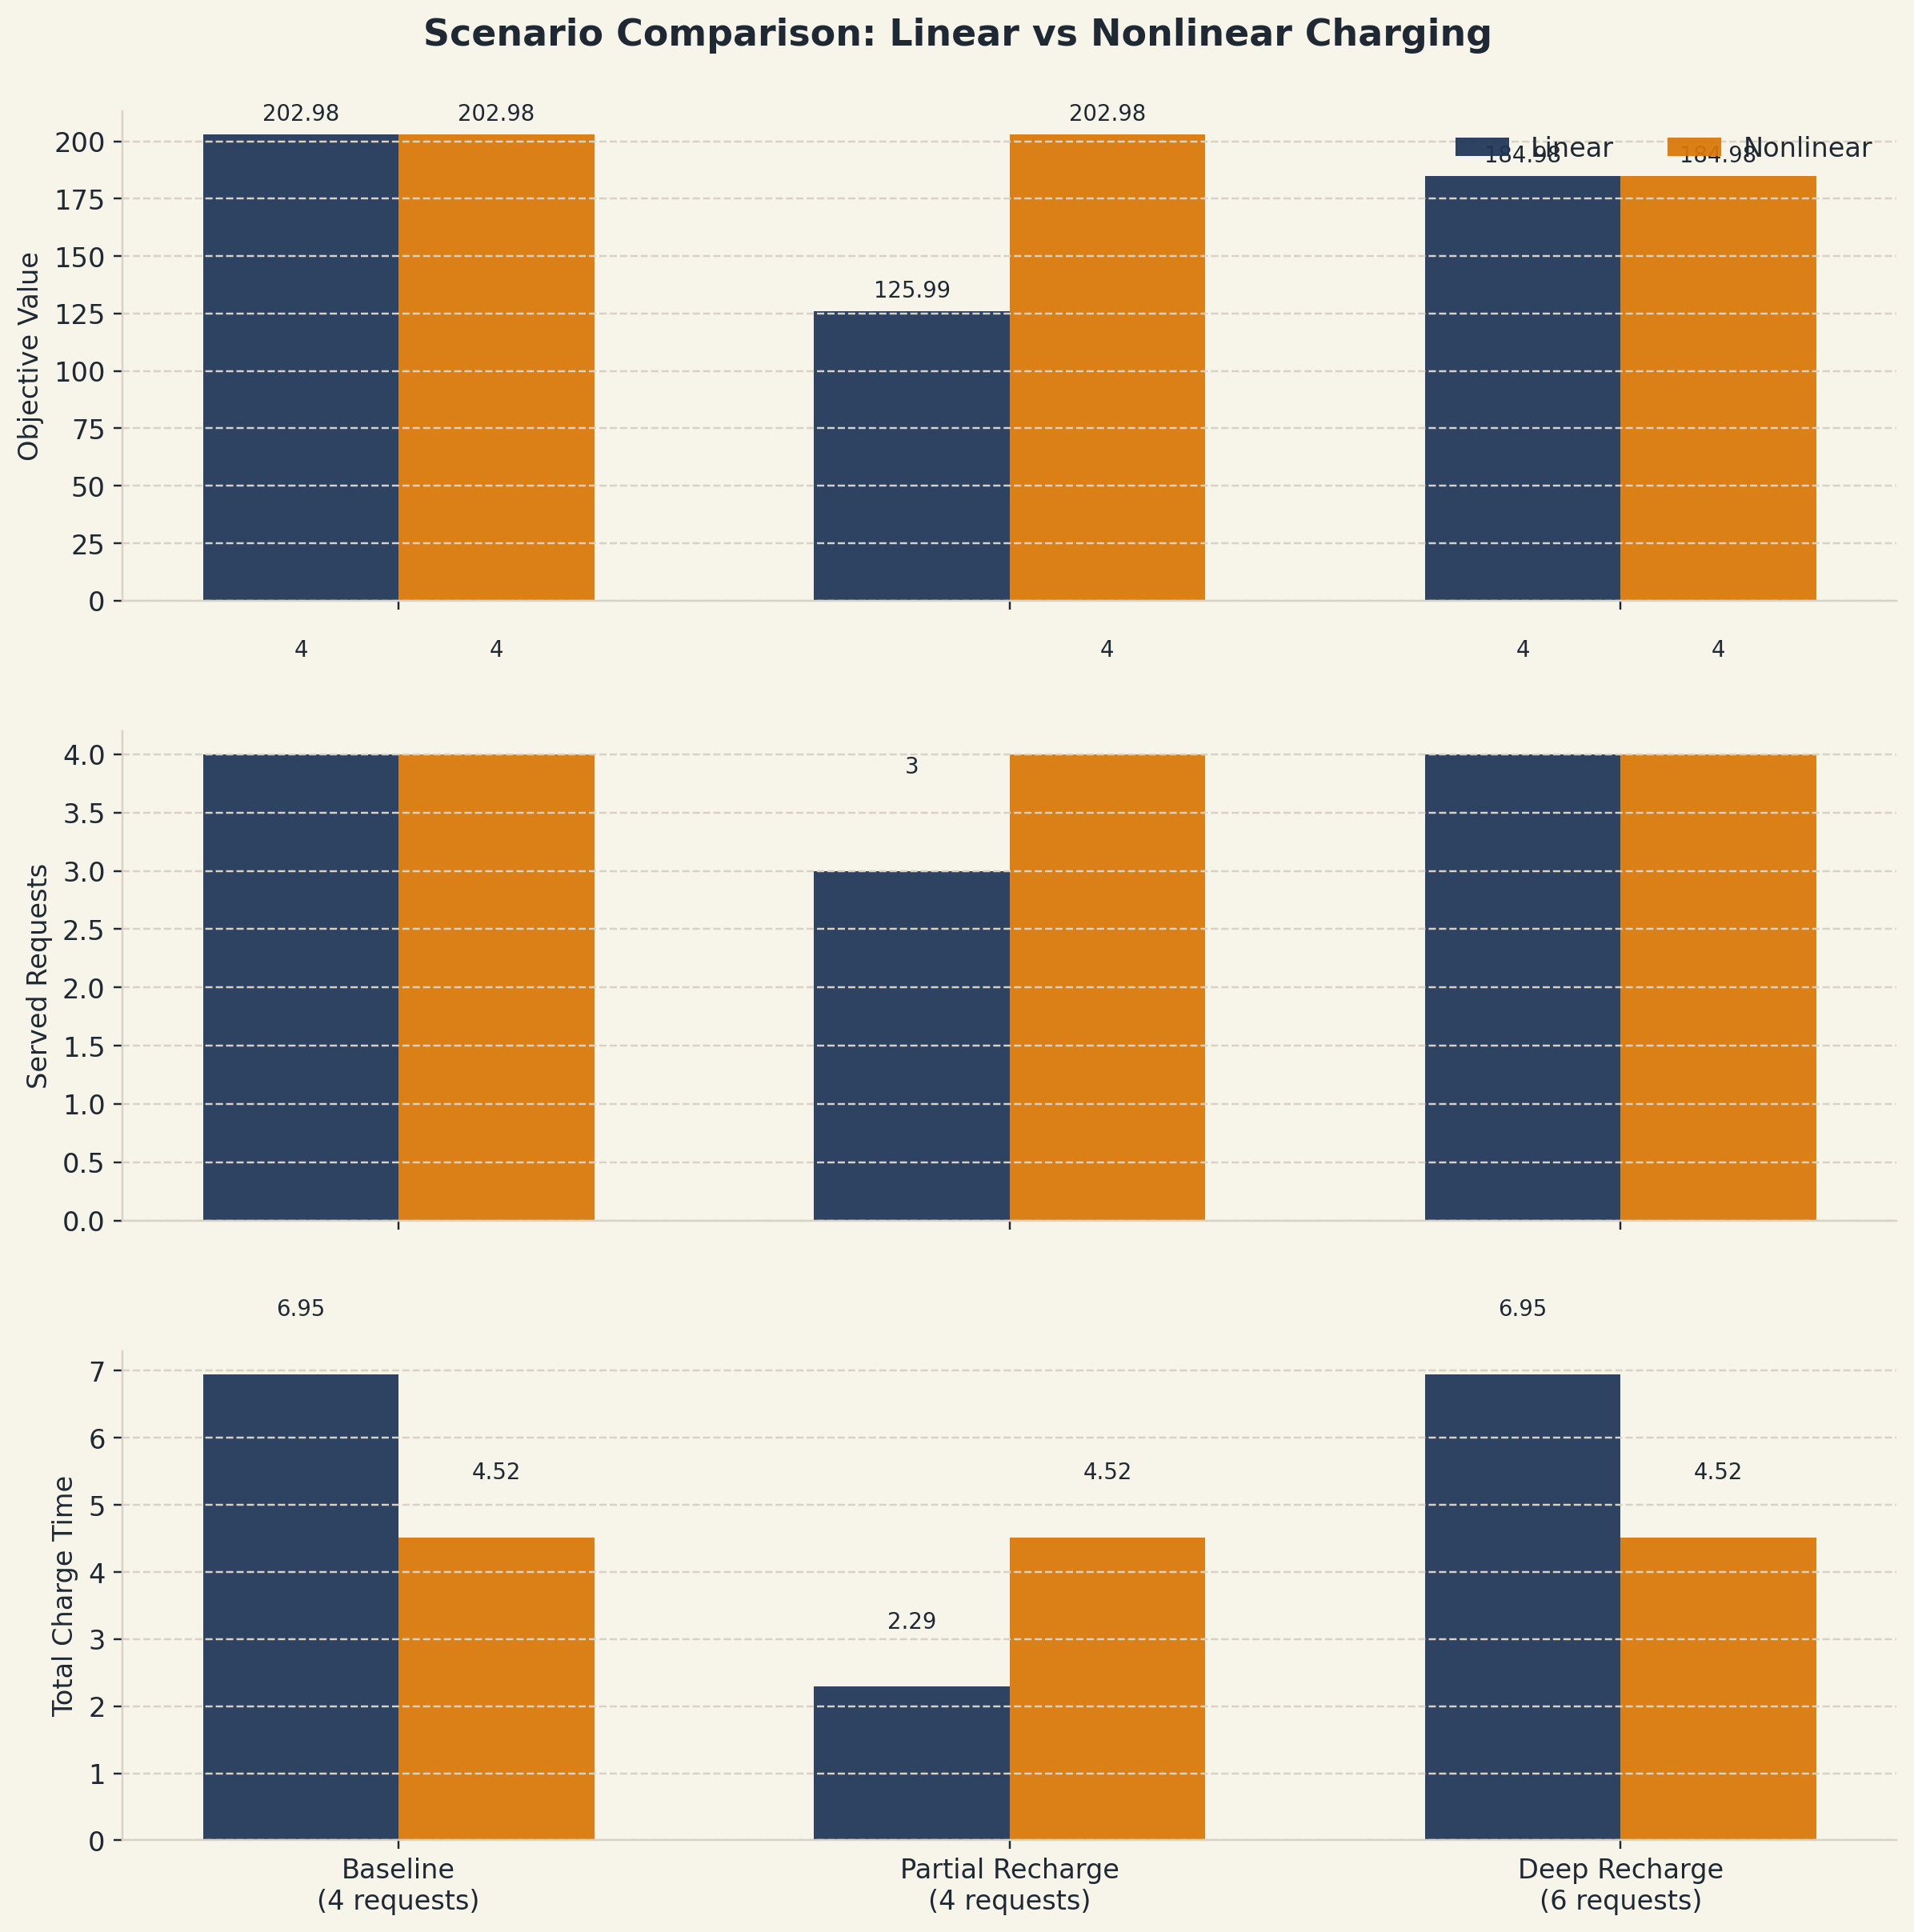
\includegraphics[width=\linewidth]{scenario_comparison.png}
\\[2pt]
{\scriptsize Direct comparison across three scenarios.}

\column{0.5\textwidth}
\centering
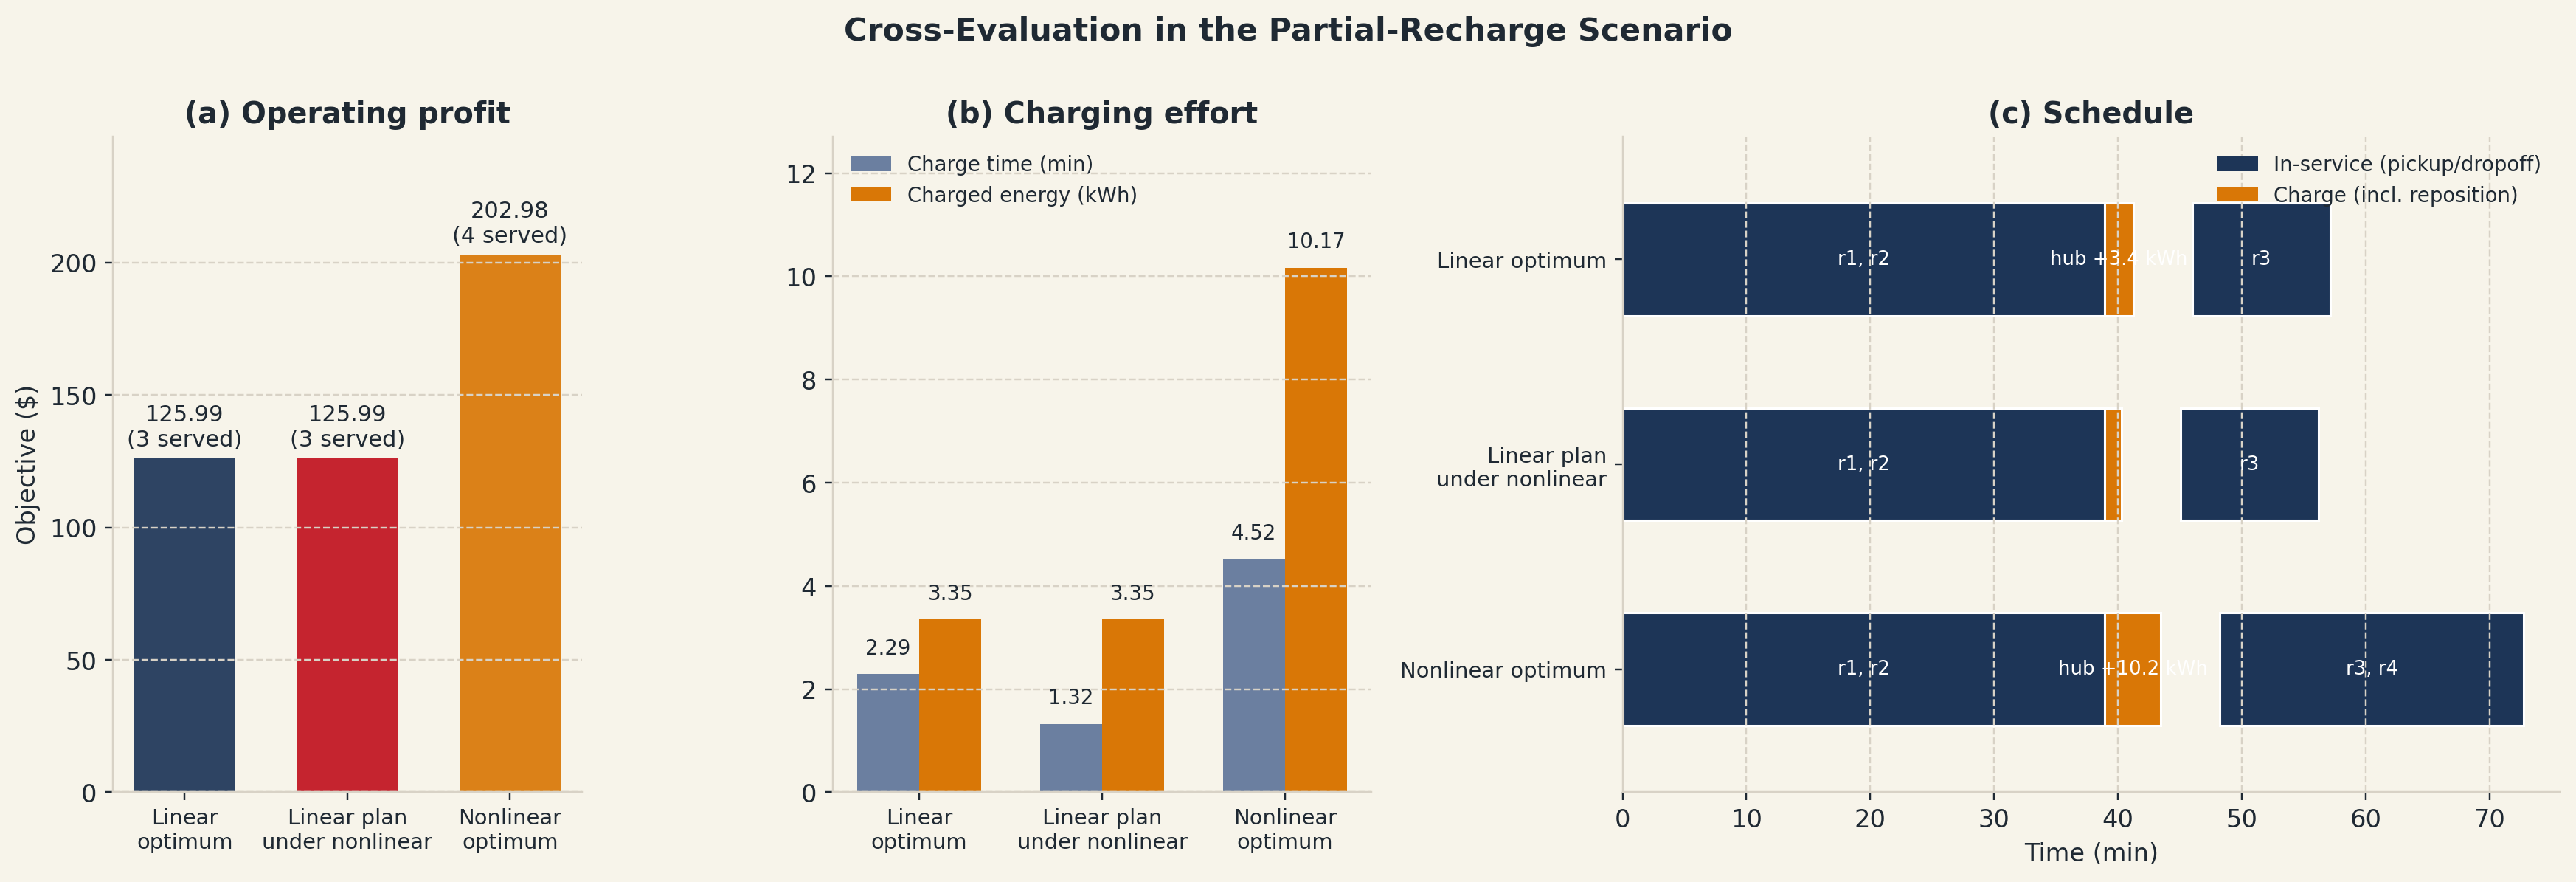
\includegraphics[width=\linewidth]{partial_recharge_cross_evaluation.png}
\\[2pt]
{\scriptsize Partial-recharge cross-evaluation: linear plan $\to$ nonlinear.}
\end{columns}
\end{frame}

% ================= STATION / DEEP RECHARGE =================
\begin{frame}{Station Choice and the Deep-Recharge Regime}
\begin{columns}[T,onlytextwidth]
\column{0.55\textwidth}
\textbf{Station selection is actively used}
\begin{itemize}\itemsep2pt
  \item Dispatch from \texttt{depot} (cheap, slower) for Trip 1.
  \item Recharge at \texttt{hub} (fast, pricier) between trips --- the hub's short time scale is worth its higher \$/kWh because it unlocks tight time windows.
  \item Confirms that both the \emph{initial-station} and \emph{mid-plan-station} decision layers bind on the optimum.
\end{itemize}

\textbf{Deep recharge at $R=5$: honest negative result}
\begin{itemize}\itemsep2pt
  \item Both modes serve \{\texttt{r1..r4}\}, drop \texttt{r5}, charge the same 10.17 kWh.
  \item Objective drop $202.98 \to 184.98 = -18$ (exactly the unserved-request penalty).
  \item The taper does \emph{not} always discriminate --- it discriminates \emph{only when} the constant-rate charge time is what creates the feasibility collision.
\end{itemize}

\column{0.43\textwidth}
\centering
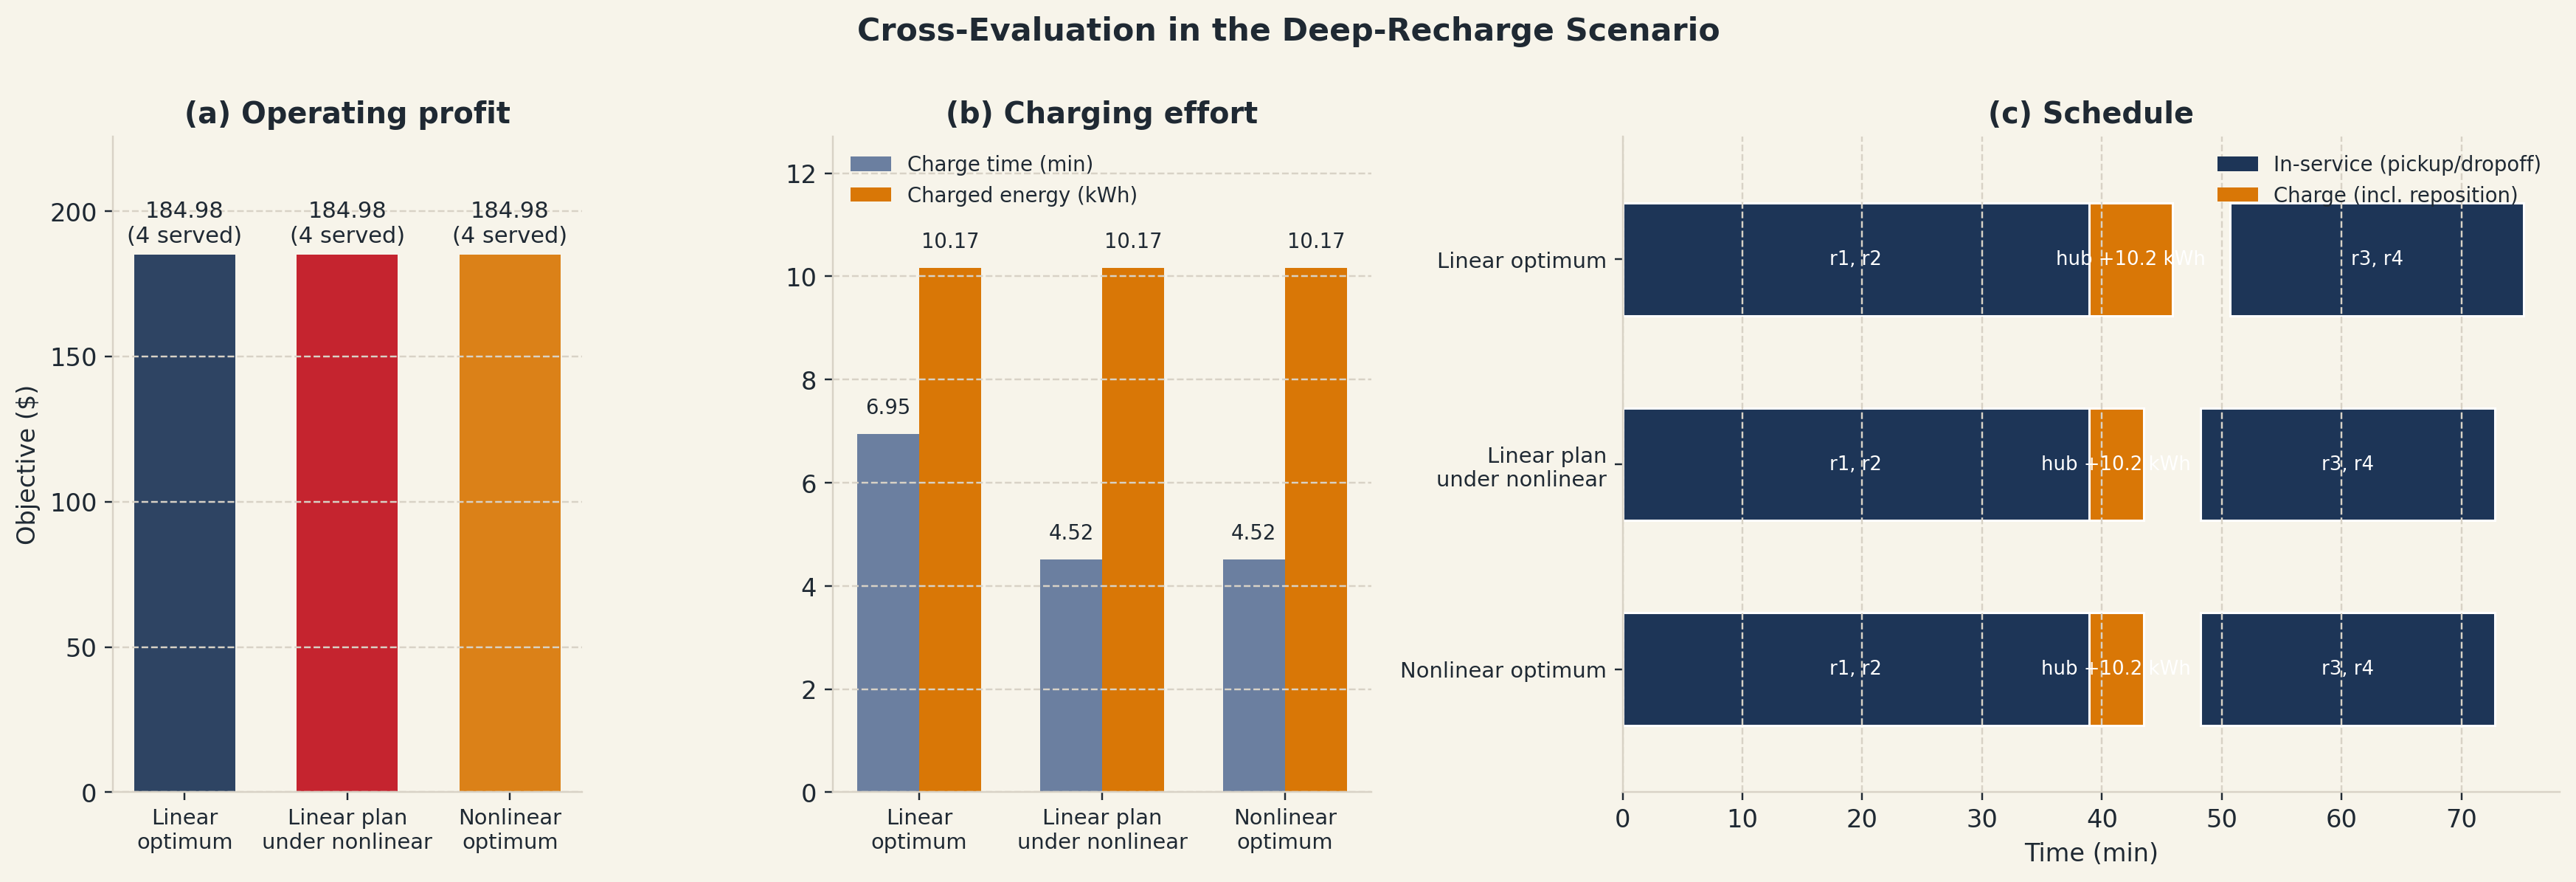
\includegraphics[width=\linewidth]{deep_recharge_cross_evaluation.png}
\\[2pt]
{\scriptsize Deep-recharge cross-evaluation.}
\end{columns}
\end{frame}

\section{Takeaways}

% ================= TAKEAWAY =================
\begin{frame}{Main Takeaways}
\begin{block}{Operational implication}
Charging realism is \textbf{state-dependent}, not monotone: the tapering assumption changes \emph{which} requests get served when, and only when, the constant-rate charge time would collide with a service time window.
\end{block}

\vspace{4pt}
\textbf{What we showed}
\begin{itemize}\itemsep2pt
  \item A one-stage integrated MIP can handle multi-station charging, station-specific speed \& price, dispatch-station decisions, and a nonlinear charging profile --- \emph{without} the bilinear $E = p\,\theta$ term, by absorbing $p$ into a station-specific time-axis scaling of a shared PWL.
  \item In partial recharge: \alert{nonlinear $\to$ +1 served request, +76.99 profit, while the linear-optimal plan remains feasible but leaves revenue on the table}.
  \item Symmetric cross-evaluation: \alert{the nonlinear-optimal plan is \textbf{infeasible} under linear charging}. Using a simplified linear model risks producing a plan the battery cannot execute.
  \item In deep recharge at $R=5$: both models agree --- negative-but-honest result.
\end{itemize}
\end{frame}

% ================= LIMITATIONS + NEXT =================
\begin{frame}{Limitations \& Next Steps}
\textbf{Limitations}
\begin{itemize}\itemsep2pt
  \item PWL approximation, not the explicit bilinear form (intentional tractability trade).
  \item Synthetic instances; no calibration against a published benchmark.
  \item Current Gurobi pip license forces small instances (1 bus, up to 5 requests).
  \item Static planning; no dynamic / stochastic requests.
\end{itemize}

\vspace{4pt}
\textbf{Natural next steps}
\begin{itemize}\itemsep2pt
  \item Rerun deep recharge at $R=6$ once a full license is available --- this is where we expect the opposite asymmetry (linear-optimal overcommits under nonlinear) to finally materialize.
  \item Stations-many-buses scaling with a decomposition or column-generation wrapper.
  \item Sensitivity sweep on \{battery capacity, time-window width, station price ratio\}.
\end{itemize}
\end{frame}

% ================= QUESTIONS =================
{
\setbeamercolor{background canvas}{bg=PurdueBlack}
\begin{frame}[plain]
\vfill
\begin{center}
{\Huge\color{PurdueGold}\textbf{Thank you}}\\[10pt]
{\large\color{white} Questions?}\\[30pt]
{\footnotesize\color{PurdueGold} Yang Li \quad $\cdot$ \quad Xiao Li \quad $\cdot$ \quad IE 538 $\cdot$ Spring 2026}
\end{center}
\vfill
\end{frame}
}

% ================= BACKUP SLIDES =================
\begin{frame}{Backup --- Model Size \& Solver Settings}
\centering\small
\begin{tabular}{@{}ll@{}}
\toprule
\textbf{Item} & \textbf{Value} \\
\midrule
Solver & Gurobi 11 (pip license, restricted size) \\
Modelling API & \texttt{gurobipy} Python \\
Charging PWL & \texttt{addGenConstrPWL} (general constraint) \\
Station-off coupling & \texttt{addGenConstrIndicator} \\
Multi-objective & Hierarchical: profit (prio 2) $\succ$ time (prio 1) \\
Symmetry breaking & Lex-order on \texttt{bus\_used} and \texttt{trip\_active} \\
\midrule
Scenario runtime & 0.08--0.56 s per solve on a laptop CPU \\
MIP gap at termination & 0 (solved to optimality) \\
\bottomrule
\end{tabular}

\vspace{10pt}
\textbf{Big-$M$ values (tightened per constraint family)}
\begin{itemize}\itemsep1pt
  \item $M_{\text{time}} = T_{\text{hor}} + \theta_{\max} + \tau_{\max}^{\text{leg}}$
  \item $M_{\text{energy}} = \overline{L} + e_{\max}^{\text{leg}}$
  \item $M_{\text{load}} = C_b + n_{\max}$
\end{itemize}
\end{frame}

\begin{frame}{Backup --- Constraint Families (Abbreviated)}
\scriptsize
\begin{columns}[T,onlytextwidth]
\column{0.48\textwidth}
\textbf{Request \& trip logic}\\
$y_q=\sum_{k,r}y_{kqr}$, \quad $u_{k,r+1}\le u_{kr}$,\\
$y_{kqr}\le u_{kr}$,\\
one-first + one-last: $\sum_i l^{\text{first}}_{kir}=u_{kr}=\sum_i l^{\text{last}}_{kir}$.

\vspace{4pt}
\textbf{Routing + time windows}\\
in/out degree through $x_{kijr}$, first/last indicators;\\
$t_{1,q}\le a_{k,q^o,r}\le t_{2,q}$ (with big-$M$);\\
$a_{kjr}\ge a_{kir}+\tau_{ij}-M(1-x_{kijr})$.

\vspace{4pt}
\textbf{Battery within trip}\\
$L_{kjr}=L_{kir}-e_{ij}$ along active arcs;\\
$\underline L \le L_{kir},L^{\text{start}}_{kr},L^{\text{end}}_{kr} \le \overline L$.

\column{0.48\textwidth}
\textbf{Inter-trip charging (the nonlinear core)}\\
Choose one station: $\sum_s z_{ksr}=u_{k,r+1}$.\\
$E_{ksr}=\mathrm{PWL}_s(\theta_{ksr})$ (via \texttt{addGenConstrPWL}).\\
Indicator: $z_{ksr}=0 \Rightarrow \theta_{ksr}=E_{ksr}=0$.\\
$L^{\text{start}}_{k,r+1}=L^{\text{end}}_{kr}-e^{\text{return}}+E_{ksr}-e^{\text{start}}$.

\vspace{4pt}
\textbf{Initial-station decision}\\
$\sum_s \sigma_{ks}=u_{k,1}$; link $\sigma_{ks}$ to the first-trip first node through aggregated equalities, drive the first-leg time and energy.

\vspace{4pt}
\textbf{Symmetry \& sub-objective}\\
$\mathrm{bus\_used}[k_i]\ge\mathrm{bus\_used}[k_{i+1}]$;\\
$\min\sum_{k,r}(T^{\text{start}}_{kr}+T^{\text{end}}_{kr})$ as secondary objective.
\end{columns}
\end{frame}

% ================= BACKUP: NOTATION =================
\begin{frame}{Backup --- Key Notation}
\scriptsize
\begin{columns}[T,onlytextwidth]
\column{0.48\textwidth}
\textbf{Sets}
\begin{tabular}{@{}ll@{}}
$K$ & Buses, index $k$ \\
$R$ & Trip slots per bus, index $r$ \\
$Q$ & Requests, index $q$ \\
$S$ & Charging stations, index $s$ \\
$N = N^o \cup N^d$ & Pickup / drop-off nodes \\
\end{tabular}

\vspace{4pt}
\textbf{Binary decisions}
\begin{tabular}{@{}ll@{}}
$y_q$        & 1 if request $q$ served \\
$y_{kqr}$    & 1 if bus $k$ serves $q$ in trip $r$ \\
$u_{kr}$     & 1 if bus $k$ operates trip $r$ \\
$x_{kijr}$   & 1 if arc $i\!\to\!j$ used \\
$l^{\text{first}}_{kir},l^{\text{last}}_{kir}$ & First / last node of the trip \\
$z_{ksr}$    & 1 if bus $k$ charges at $s$ between trips \\
$\sigma_{ks}$& 1 if bus $k$ dispatches from station $s$ \\
\end{tabular}

\column{0.48\textwidth}
\textbf{Continuous decisions}
\begin{tabular}{@{}ll@{}}
$a_{kir}$               & Arrival time at node \\
$w_{kir}$               & Onboard load after node \\
$L_{kir}$               & Battery level after node \\
$L^{\text{start}}_{kr},L^{\text{end}}_{kr}$ & Battery at trip boundaries \\
$T^{\text{start}}_{kr},T^{\text{end}}_{kr}$ & Trip start / end time \\
$\theta_{ksr}$          & Charging duration \\
$E_{ksr}$               & Acquired energy \\
\end{tabular}

\vspace{4pt}
\textbf{Parameters (highlights)}
\begin{tabular}{@{}ll@{}}
$C_m,C_z,C_e,C_d,C_v,C_t$ & Revenue / penalty / charge / travel / fleet / trip costs \\
$\overline L,\underline L$  & Battery upper / lower bound \\
$C_b$                     & Passenger capacity \\
$t_{1,q},t_{2,q}$         & Pickup window for $q$ \\
$\tau_{ij},e_{ij}$        & Travel time / energy $i\to j$ \\
$\mathrm{PWL}_s(\cdot)$   & Station-$s$ charging curve \\
\end{tabular}
\end{columns}
\end{frame}

% ================= BACKUP: ANTICIPATED Q&A =================
\begin{frame}{Backup --- Anticipated Questions}
\small
\begin{block}{Q1. Why not keep the bilinear $E = p\,\theta$?}
Our implementation factors station-specific $p_s$ into the \emph{time-axis scaling} of a shared PWL curve. Gurobi's \texttt{addGenConstrPWL} then enforces $E = f_s(\theta)$ exactly on the approximation. This keeps the model MIP (not MINLP) while preserving the key nonlinear effect --- the tapering shape of the curve.
\end{block}

\begin{block}{Q2. Is the PWL approximation tight?}
The taper uses 6 segments on $[0,32]$; slopes step from 2.08 down to 0.18 kWh/min, giving a piecewise upper envelope of a typical Li-ion SoC-vs-time curve. Finer grids are cheap (only one additional breakpoint per segment), but the course-size instance already terminates at MIP gap 0.
\end{block}

\begin{block}{Q3. Why does deep recharge at $R{=}5$ show no asymmetry?}
At $R{=}5$ both models drop \texttt{r5} and share the same 2-trip plan with the same 10.17 kWh recharge --- time windows are loose enough that neither the 6.95 min (linear) nor the 4.52 min (nonlinear) recharge collides. The opposite asymmetry (linear over-commits) is expected at $R{=}6$, which exceeds our current Gurobi pip license.
\end{block}
\end{frame}

\begin{frame}{Backup --- Anticipated Questions (cont.)}
\small
\begin{block}{Q4. Why pick the hub station when it charges pricier?}
Hub costs \$0.64/kWh vs.\ depot \$0.48/kWh, but its time-scale factor is 0.82 (vs.\ depot's 1.08). In the partial-recharge regime the binding constraint is \emph{time} (r4's pickup window), not \emph{cost}, so the solver pays for speed.
\end{block}

\begin{block}{Q5. How do we know the cross-evaluation is not picking the wrong plan?}
The discrete binaries ($u_{kr},\,x_{kijr},\,l^{\text{first/last}},\,z_{ksr}$) are extracted from the source solve and re-imposed as equality bounds in the target solve. Continuous variables (arrivals, battery levels, charge time / energy) are still free --- only the routing \& station choice is fixed.
\end{block}

\begin{block}{Q6. Can this scale?}
Not directly. The model is a MIP with $O(|K||R|\,|N|^2)$ arc variables plus PWL constraints per $(k,s,r)$. A full-license experiment with \{multiple buses, 15+ requests\} would benefit from decomposition (e.g.\ column generation on trip patterns) or a rolling-horizon wrapper --- flagged as future work.
\end{block}
\end{frame}

\end{document}
